\documentclass[11pt]{article}
\usepackage[paper1]{../paper_style/kirin-papers}
\KirinSetShortTitle{Reading Ouro with J-Lens}
\hypersetup{pdftitle={Reading Ouro with J-Lens},pdfauthor={Jan Kirin}}
\setlength{\parskip}{4pt}
\setlength{\parindent}{0pt}
\begin{document}
\KirinTitleBlock
  {MATS 12.0 application}
  {Reading Ouro with J-Lens}
  {Intermediate readout across recurrent passes}
  {Jan Kirin}
  {}
  {September 2026}
  {}
\begin{abstractbox}

I tested whether J-Lens reads known intermediates from Ouro-2.6B's hidden states better than the logit lens. I care about what these readouts can tell us before the model answers. Ouro runs the same 48 layers four times. I also fitted lenses to the earlier exits and the final exit, expecting their readouts to agree more as the model kept looping. At this point I still expected to sleep.

The clearest result went against my expectation: on 90 multihop items, the logit lens wins at each of the first three loops. With 100 fitting prompts, the final-exit J-Lens minus logit-lens difference at loop 2 is −0.479, with a paired 95\% interval of [−0.579, −0.377]. This is excess hit@10: finding the intermediate somewhere in the loop, minus finding matched controls the same way. Arithmetic is mixed. J-Lens loses at loop 1 but wins at loop 2.

The local-versus-final lens gap also did not steadily shrink at the main readout position. Moving back one token changed that: KL then decreased, though top-1 agreement remained around 0.5\% or less. I can report the disagreement, but not a general failure to converge, and certainly not that either lens tells me exactly what the model is doing.

My guess is that training every Ouro loop through the same output head helps the logit lens. I haven't tested that explanation. One model, small nested fits, no tuned lens yet, and no causal test of the labelled intermediates.


\end{abstractbox}
\begin{minipage}{\linewidth}
\centering
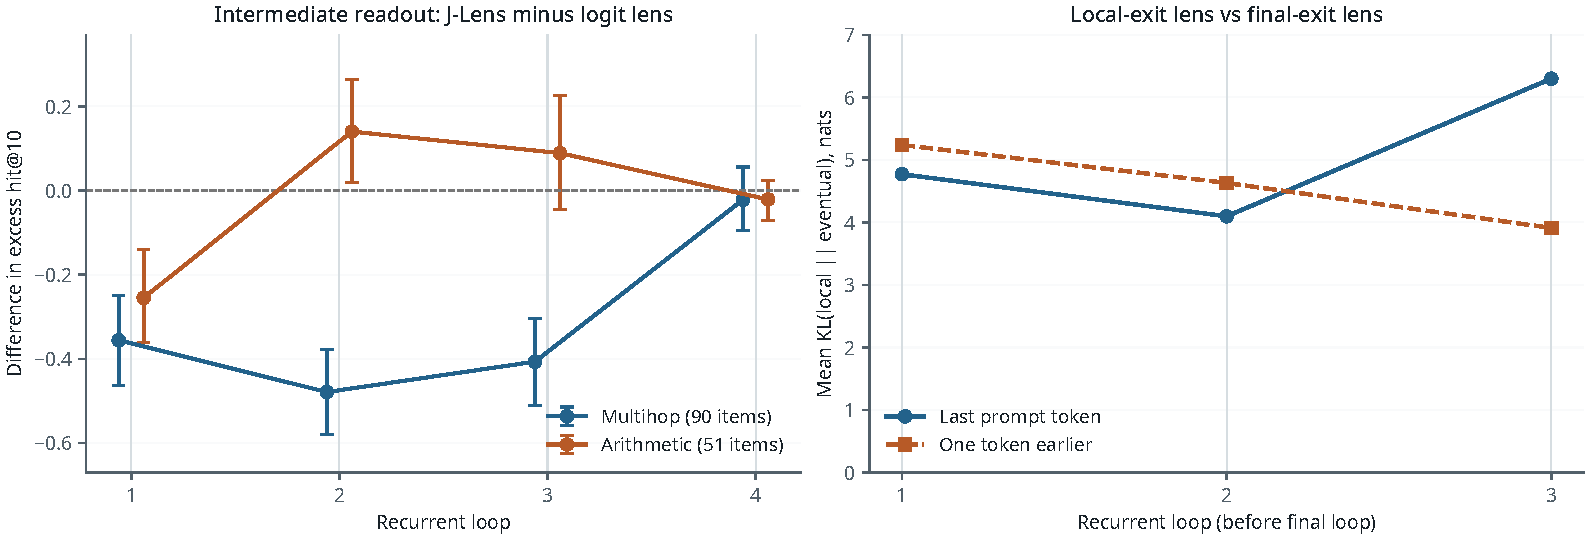
\includegraphics[width=\linewidth]{../figures_for_doc/application_results.pdf}
\raggedright
\kirinfigcaption{Figure 1.}{Lenses fitted on 100 prompts. Left: J-Lens minus logit lens, with unadjusted 95\% item-bootstrap intervals. Below zero favours the logit lens. Right: local-versus-final lens KL over 148 prompts and 48 layers, evaluated on the laptop using the saved lenses. The trend changes with token position.}
\end{minipage}
\clearpage
\section{Some actual examples}

Five randomly sampled examples from the earlier local evaluation, drawn from 142 eligible items. “Intermediate” is the task label, not proof that the model uses it. Surrounding whitespace is trimmed; row four has its line breaks written out.


\begin{center}
\small
\begin{tabularx}{\linewidth}{@{}>{\raggedright\arraybackslash}X>{\raggedright\arraybackslash}p{.22\linewidth}>{\raggedright\arraybackslash}p{.24\linewidth}@{}}
\toprule
\rowcolor{KirinAccentPale} {\sffamily\bfseries Prompt} & {\sffamily\bfseries Intermediate → target} & {\sffamily\bfseries Model continuation} \\
\midrule
Fact: The chemical symbol for the element with atomic number 26 is & iron → Fe & Fe. \\
Fact: One more than the number whose name rhymes with hive is & five → 6 & 100. \\
10 + 5 - 3 = & 15 → 12 & 12 \\
((1 + 2) * 3) - 4 = & 9 → 5 & 9 [two newlines] (( \\
ten minus two times three equals & 6 → four & Answer: \\
\bottomrule
\end{tabularx}
\end{center}

On the iron item, J-Lens's best vocabulary rank in loop 1 is 979; the logit lens puts it first. On the nested arithmetic item, reading “9” could just mean reading the wrong answer. Worth keeping in mind before calling these internal reasoning steps. Across all 148 items, 72 continuations pass the corrected answer check.

\section{J-Lens against the logit lens}

The first question was whether the Jacobian adds anything useful. I recorded hidden states at all 192 loop/layer locations and fitted the released estimator on Wikitext, averaging Jacobians over fitting prompts and valid token positions. The logit lens applies the model's output readout directly. It is the comparison that matters here, because an intermediate appearing in a lens is less interesting if the output head already reads it.

The released tasks contain 93 multihop and 55 arithmetic items. Excluding leaked or unscorable intermediates leaves 90 multihop items with 100 labels and 51 numeric arithmetic items. At the last prompt token, I check whether the intermediate is in the top ten at any layer and subtract the mean of the identical test over same-kind control names. Multiple labels are averaged within an item first. The eight intervals below use 20,000 paired item-bootstrap draws and are unadjusted.

Final-exit J-Lens minus logit lens, with 100 fitting prompts:


\begin{center}
\small
\begin{tabularx}{\linewidth}{@{}>{\raggedright\arraybackslash}Xcccc@{}}
\toprule
\rowcolor{KirinAccentPale} {\sffamily\bfseries Population} & {\sffamily\bfseries Loop 1} & {\sffamily\bfseries Loop 2} & {\sffamily\bfseries Loop 3} & {\sffamily\bfseries Loop 4} \\
\midrule
Multihop & −0.356 & −0.479 & −0.407 & −0.022 \\
95\% interval & [−0.463, −0.249] & [−0.579, −0.377] & [−0.510, −0.304] & [−0.096, +0.056] \\
Arithmetic & −0.255 & +0.140 & +0.089 & −0.021 \\
95\% interval & [−0.362, −0.139] & [+0.020, +0.264] & [−0.045, +0.226] & [−0.072, +0.024] \\
\bottomrule
\end{tabularx}
\end{center}

I increased the fit from 8 to 100 prompts to check whether the weak early readout was just too little fitting data. It did not recover over that range. These are nested fits, though, so I still need independent repeats. Arithmetic loop 2 is also a real qualification: its interval favours J-Lens. “J-Lens is worse” would be too broad.

A separate supervised probe on \texttt{(a + b) * c} gives another comparison. After keeping mirror pairs together and excluding labels absent from a training fold, 576 prompts remain. Loop-1 held-out accuracy is 0.594 for the probe, 0.764 for the logit lens and 0.392 for J-Lens; majority baseline 0.125. This uses an older lens with incomplete fitting records, so I keep it separate from the 100-prompt rerun.

\clearpage
\section{Changing the exit changes what gets read}

I wanted to know whether a lens aimed at the final exit gives the same picture as one aimed at the current loop's exit. Fitted all four on 100 prompts and compared them at the same hidden states. If their gap shrank with depth, that would support the convergence I expected.

At the main position, mean KL(local \ensuremath{\Vert} final) is 4.77, 4.10 and 6.30 nats at loops 1–3, averaged over all 148 prompts and 48 layers. Top-1 agreement over the last eight layers is at most 3.3\%. This is disagreement between two lens distributions, not a measurement of which one is faithful to the model.

Then the position control changes the interpretation. One token earlier, KL is 5.24, 4.63 and 3.91, so it does decrease. Top-1 agreement stays around 0.5\% or less. The gap is large at both positions, but the trend is position-sensitive. I can't turn that into a general claim about recurrence failing to converge.

\section{What I checked, and what is still open}

I checked the code, raw prompts and continuations, plots, and reported numbers against the saved outputs. Fable also checked the code. In the retained local checks, recording matches the ordinary model computation exactly on all 18 required comparisons. The headline effects and intervals were recomputed from the saved arrays during the write-up.

The checks found actual problems. Controls were originally averaged before taking their best layer, while each true intermediate got its own best layer. That inflated the excess score; fixed. The probe split leaked mirrored operand pairs; fixed. The answer matcher accepted “11” for “1”; fixed. A claim about directly measured single-prompt Jacobian norms was retracted because the values were modeled scatter.

The shared-head explanation is still a guess. I would next add a tuned lens, repeat fits independently, compare how the Jacobians are estimated and averaged, and test a matched model without the same per-loop supervision. I also haven't shown that the labelled intermediates are causally used. Those are open questions, not conclusions from this run.

\section{The overnight part}

The plan was to rent a GPU, sleep, and wake up to results. I left Claude Opus overseeing it. Both I and the session went to sleep. The pod did not. About \$52 later, nothing was retrieved. Billing had no such difficulties.

After rebuilding the controller, the rerun took nine launches. Nine. The successful one initially needed about 29 minutes per fitting prompt. It was trying to use 192 CPU threads; limiting it to eight brought that down to roughly 40 seconds. Apparently most of the threads were supervising. The GPU and I are on speaking terms now. Barely.

All four 100-prompt lenses finished. The final-exit and fit-size results were recovered from the rental. The all-exit results weren't saved before timeout, so I reran that evaluation on the laptop using the saved lenses.

About 15 active hours by my estimate, excluding rental setup, waiting for fits and the form. The write-up happened during the final overnight run. Not recommended. Not the plan either.

Agents were used mainly for run supervision and launch debugging. I checked their output myself; Fable also reviewed the code, and Codex helped with later checking, editing and LaTeX.
\end{document}
